\chapter{Deformed Nuclei}

\section{Nuclear deformation}

Most of the nuclei across the nuclide chart are spherical or symmetric in their ground state. Moreover, for the axially symmetric nuclei (i.e, either \emph{oblate} or \emph{prolate}), there is a prolate over oblate dominance.
% \begin{figure}[ht]
%     \centering
%     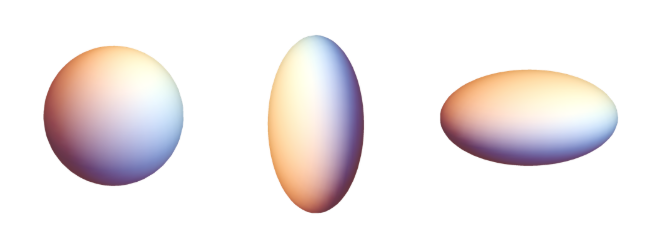
\includegraphics[scale=0.3]{Chapters/Figures/nuclear_shapes.png}
%     \caption{Nuclear Shapes.}
%     \label{nuclear_shapes}
% \end{figure}

The spherical shell model only describes nuclei near the closed shells. On the other side, for the nuclei that lie far from closed shells, a deformed potential must be employed. 
\par In the case of even-even nuclei, unique band structures resulting from the vibrations and rotations of the nuclear surface (as proposed by Bohr and Mottelson \cite{bohr1998nuclear} in the \emph{Geometric Collective Model} - GCM) appear in the energy range 0-2 MeV.

Within the GCM, the nucleus is described as a classical charged liquid drop. For the low-lying energy spectrum, usually, the compression of nuclear matter and the nuclear skin thickness are neglected. This results in the final picture of a liquid drop with a constant nuclear density and a sharp surface \cite{greiner1996nuclear}.

\subsection{Collective coordinates}

The nuclear surface can be described via an expansion of the spherical harmonic functions with some time-dependent parameters as \emph{expansion coefficients}. The expression of the nuclear shape is shown below \cite{greiner1996nuclear}:
\begin{align}
    R(\theta,\varphi,t)=R_0\left(1+\sum_{\lambda=0}^\infty\sum_{-\lambda}^\lambda\alpha_{\lambda\mu}(t)Y_\lambda^\nu(\theta,\varphi)\right)\ .
    \label{nuclear-shape}
\end{align}

In \ref{nuclear-shape}, $R$ denotes the nuclear radius as a function of the spherical coordinates $\theta,\varphi)$ expressing the direction, and the time $t$, while $R_0$ is the radius of the spherical nucleus when all the expansion coefficients vanish. It is worth mentioning that the expansion coefficients $\alpha_{\lambda\mu}$ act as \emph{collective coordinates} since the time-dependent amplitudes describe the vibrations of the nuclear surface.

\subsection{Nuclear radius under rotation}

To get a grasp at the physical meaning behind the deformation parameters that are used to describe the nuclear surface, it is instructive to see what happens when the system undergoes a rotation transformation.

The function $R(\theta,\varphi)$ describes the original (non-rotated) nuclear shape. Rotating the system will result in the change of the angular coordinates $(\theta,\varphi)$ to $(\theta',\varphi')$, which will correspond to a new function $R'(\theta',\varphi')$. Moreover, both nuclear surfaces (i.e., the non-rotated and the rotated one) must hold the equality:
\begin{align}
    R'(\theta',\varphi')=R(\theta,\varphi)
\end{align}

The rotational invariance of $R$ employs that $R'(\theta,\varphi)$ must have the same functional form, but the expansion coefficients $\alpha_{\lambda\mu}$ must be rotated, meaning:
\begin{align}
    \sum_{\lambda\mu}\alpha_{\lambda\mu}'Y'_{\lambda\mu}(
        \theta,\varphi)
\end{align}